\documentclass[margin,line]{res}
\usepackage{hyperref}
\usepackage{url}
\usepackage{graphicx}
\oddsidemargin -.5in
\evensidemargin -.5in
\textwidth=6.0in
\itemsep=0in
\parsep=0in
\topmargin=0in
\topskip=0in
 
\newenvironment{list1}{
  \begin{list}{\ding{113}}{%
      \setlength{\itemsep}{0in}
      \setlength{\parsep}{0in} \setlength{\parskip}{0in}
      \setlength{\topsep}{0in} \setlength{\partopsep}{0in}
      \setlength{\leftmargin}{0.17in}}}{\end{list}}
\newenvironment{list2}{
  \begin{list}{$\bullet$}{%
      \setlength{\itemsep}{0in}
      \setlength{\parsep}{0in} \setlength{\parskip}{0in}
      \setlength{\topsep}{0in} \setlength{\partopsep}{0in}
      \setlength{\leftmargin}{0.2in}}}{\end{list}}


    
\begin{document}

\name{\LARGE NIKHILESH MATH} \hfill {\em \today}

\begin{resume}
\section{\sc Contact Information}

\vspace{.05in}
\begin{tabular}{@{}p{3.5in}p{3in}}
\#241,5th main road,             & {Phone:}  +91 7676301776 \\
3rd Block Thyagaraja Nagar 
 & {E-mail:}  nikhileshm9@gmail.com\\
Bengaluru - 560028.\\
 & 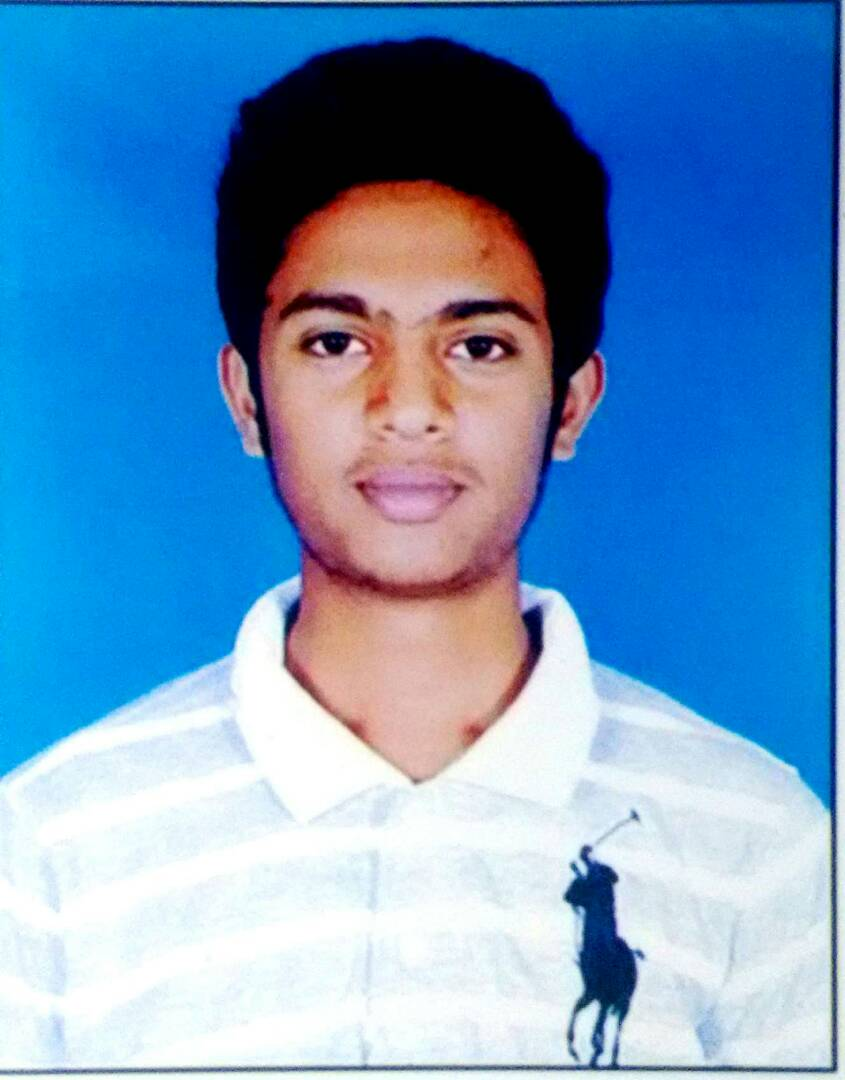
\includegraphics[width=5cm]{PassportPhoto}
\end{tabular}
\section{\sc Objective}

Seeking an internship position as a part of eYSIP - 2017 at Indian Institute of Technology,Bombay to explore career options in the Embedded Research Sector . A hard-working and self-motivated undergraduate student in 3rd year Electronics and Communication.

\section{\sc Education}
\begin{tabular}{ L{1in} L{1in} L{1in} L{0.5in} L{1in} }
	\textbf{Degree} & \textbf{College/School} & \textbf{University} & \textbf{Passing Year} & \textbf{Pass Percentage} \\ 
	\hline \\
	B.E(ECE) & B.M.S College & Visvesvaraya  & 2018 & 8.32 (As of Sem V) \\ &  of Engineering & Technological University & & \\ \\
	12th & Independent & Department of Pre-University & 2014 & 87\% \\ & PU College & Education, Karnataka & & \\
	10th & Nandi International& Central Board of & 2012 & 8.6 \\ &  School,Bellary & Secondary Education & & \\
	\hline	
\end{tabular}

\end{resume}
\end{document}




